% Options for packages loaded elsewhere
\PassOptionsToPackage{unicode}{hyperref}
\PassOptionsToPackage{hyphens}{url}
\PassOptionsToPackage{dvipsnames,svgnames*,x11names*}{xcolor}
%
\documentclass[
]{article}
\usepackage{lmodern}
\usepackage{amssymb,amsmath}
\usepackage{ifxetex,ifluatex}
\ifnum 0\ifxetex 1\fi\ifluatex 1\fi=0 % if pdftex
  \usepackage[T1]{fontenc}
  \usepackage[utf8]{inputenc}
  \usepackage{textcomp} % provide euro and other symbols
\else % if luatex or xetex
  \usepackage{unicode-math}
  \defaultfontfeatures{Scale=MatchLowercase}
  \defaultfontfeatures[\rmfamily]{Ligatures=TeX,Scale=1}
\fi
% Use upquote if available, for straight quotes in verbatim environments
\IfFileExists{upquote.sty}{\usepackage{upquote}}{}
\IfFileExists{microtype.sty}{% use microtype if available
  \usepackage[]{microtype}
  \UseMicrotypeSet[protrusion]{basicmath} % disable protrusion for tt fonts
}{}
\makeatletter
\@ifundefined{KOMAClassName}{% if non-KOMA class
  \IfFileExists{parskip.sty}{%
    \usepackage{parskip}
  }{% else
    \setlength{\parindent}{0pt}
    \setlength{\parskip}{6pt plus 2pt minus 1pt}}
}{% if KOMA class
  \KOMAoptions{parskip=half}}
\makeatother
\usepackage{xcolor}
\IfFileExists{xurl.sty}{\usepackage{xurl}}{} % add URL line breaks if available
\IfFileExists{bookmark.sty}{\usepackage{bookmark}}{\usepackage{hyperref}}
\hypersetup{
  colorlinks=true,
  linkcolor=blue,
  filecolor=Maroon,
  citecolor=Blue,
  urlcolor=Blue,
  pdfcreator={LaTeX via pandoc}}
\urlstyle{same} % disable monospaced font for URLs
\usepackage{graphicx}
\makeatletter
\def\maxwidth{\ifdim\Gin@nat@width>\linewidth\linewidth\else\Gin@nat@width\fi}
\def\maxheight{\ifdim\Gin@nat@height>\textheight\textheight\else\Gin@nat@height\fi}
\makeatother
% Scale images if necessary, so that they will not overflow the page
% margins by default, and it is still possible to overwrite the defaults
% using explicit options in \includegraphics[width, height, ...]{}
\setkeys{Gin}{width=\maxwidth,height=\maxheight,keepaspectratio}
% Set default figure placement to htbp
\makeatletter
\def\fps@figure{htbp}
\makeatother
\setlength{\emergencystretch}{3em} % prevent overfull lines
\providecommand{\tightlist}{%
  \setlength{\itemsep}{0pt}\setlength{\parskip}{0pt}}
\setcounter{secnumdepth}{5}

%% pandoc-fignos: required package
\usepackage{cleveref}

%% pandoc-eqnos: disable brackets around cleveref numbers
\creflabelformat{equation}{#2#1#3}
\newlength{\cslhangindent}
\setlength{\cslhangindent}{1.5em}
\newenvironment{cslreferences}%
  {}%
  {\par}

\author{}
\date{}

\begin{document}

\hypertarget{support-vector-machines}{%
\section{Support Vector Machines}\label{support-vector-machines}}

\hypertarget{introduction}{%
\subsection{Introduction}\label{introduction}}

Suppose that we are given a collection of data made up of samples from
two different classes, and we would like to develop an algorithm that
can distinguish between the two classes. For example, given a picture
that is either a dog or a cat, we'd like to be able to say which of the
pictures are dogs, and which are cats. For another example, we might
want to be able to distinguish ``real'' emails from ``spam.'' This type
of problem is called a \emph{classification} problem.

Typically, one approaches a classification problem by beginning with a
large set of data for which you know the classes, and you use that data
to \emph{train} an algorithm to correctly distinguish the classes for
the test cases where you already know the answer. For example, you start
with a few thousand pictures labelled ``dog'' and ``cat'' and you build
your algorithm so that it does a good job distinguishing the dogs from
the cats in this initial set of \emph{training data}. Then you apply
your algorithm to pictures that aren't labelled and rely on the
predictions you get, hoping that whatever let your algorithm distinguish
between the particular examples will generalize to allow it to correctly
classify images that aren't pre-labelled.

Because classification is such a central problem, there are many
approaches to it. We will see several of them through the course of
these lectures. We will begin with a particular classification algorithm
called ``Support Vector Machines'' (SVM) that is based on linear
algebra. The SVM algorithm is widely used in practice and has a
beautiful geometric interpretation, so it will serve as a good beginning
for later discussion of more complicated classification algorithms.

Incidentally, I'm not sure why this algorithm is called a ``machine'';
the algorithm was introduced in the paper
{[}\protect\hyperlink{ref-vapnik92}{1}{]} where it is called the
``Optimal Margin Classifier'' and as we shall see that is a much better
name for it.

\hypertarget{a-simple-example}{%
\subsection{A simple example}\label{a-simple-example}}

Let us begin our discussion with a very simple dataset (see
{[}\protect\hyperlink{ref-penguins}{2}{]} and
{[}\protect\hyperlink{ref-penguindata}{3}{]}). This data consists of
various measurements of physical characteristics of 344 penguins of 3
different species: Gentoo, Adelie, and Chinstrap. If we focus our
attention for the moment on the Adelie and Gentoo species, and plot
their body mass against their culmen depth, we obtain the following
scatterplot.

\begin{figure}
\hypertarget{fig:penguins}{%
\centering
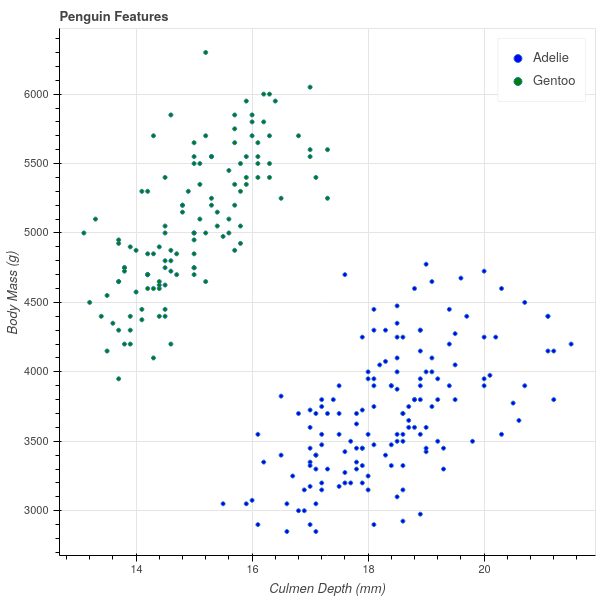
\includegraphics[width=0.5\textwidth,height=\textheight]{../img/penguins.png}
\caption{Penguin Scatterplot}\label{fig:penguins}
}
\end{figure}

Incidentally, a bird's \emph{culmen} is the upper ridge of their beak,
and the \emph{culmen depth} is a measure of the thickness of the beak.
There's a nice picture at {[}\protect\hyperlink{ref-penguindata}{3}{]}
for the penguin enthusiasts.

A striking feature of this scatter plot is that there is a clear
separation between the clusters of Adelie and Gentoo penguins. Adelie
penguins have deeper culmens and less body mass than Gentoo penguins.
These characteristics seem like they should provide a way to classify a
penguin between these two species based on these two measurements.

One way to express the separation between these two clusters is to
observe that one can draw a line on the graph with the property that all
of the Adelie penguins lie on one side of that line and all of the
Gentoo penguins lie on the other. In \cref{fig:penguinsline} I've drawn
in such a line (which I found by eyeballing the picture in
\cref{fig:penguins}). The line has the equation \[
Y = 250X+400.
\]

\begin{figure}
\hypertarget{fig:penguinsline}{%
\centering
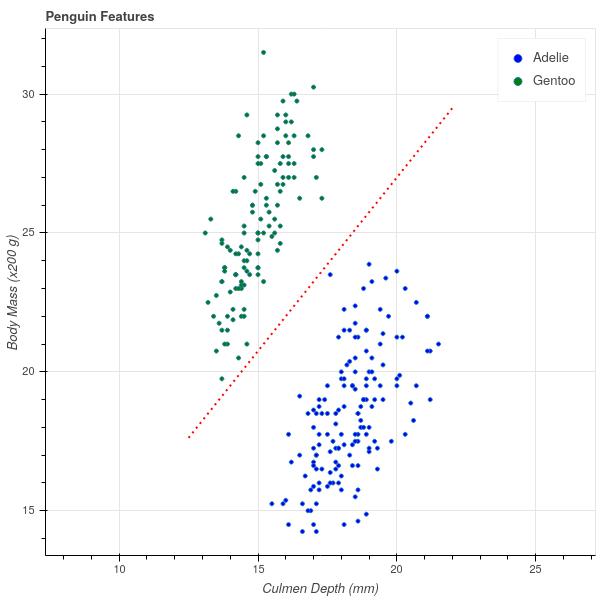
\includegraphics[width=0.5\textwidth,height=\textheight]{../img/penguins_with_line.png}
\caption{Penguins with Separating Line}\label{fig:penguinsline}
}
\end{figure}

The fact that all of the Gentoo penguins lie above this line means that,
for the Gentoo penguins, their body mass in grams is at least \(400\)
more than \(250\) times their culmen depth in mm.

\[
\mathrm{Gentoo\ mass}> 250(\mathrm{Gentoo\ culmen\ depth})+400
\]

while

\[
\mathrm{Adelie\ mass}<250(\mathrm{Adelie\ culmen\ depth})+400.
\]

Now, if we measure a penguin caught in the wild, we can compute
\(250(\mathrm{culmen\ depth})+400\) for that penguin and if this number
is greater than the penguin's mass, we say it's an Adelie; otherwise, a
Gentoo. Based on the experimental data we've collected -- the
\emph{training} data -- this seems likely to work pretty well.

\hypertarget{the-general-case}{%
\subsection{The general case}\label{the-general-case}}

To generalize this approach, let's imagine now that we have \(n\)
samples and \(k\) features (or measurements) for each sample. As before,
we can represent this data as an \(n\times k\) data matrix \(X\). In the
penguin example, our data matrix would be \(344\times 2\), with one row
for each penguin and the columns representing the mass and the culmen
depth. In addition to this numerical data, we have a classification that
assigns each row to one of two classes. Let's represent the classes by a
\(n\times 1\) vector \(Y\), where \(y_{i}=+1\) if the \(i^{th}\) sample
is in one class, and \(y_{i}=-1\) if that \(i^{th}\) sample is in the
other. Our goal is to predict \(Y\) based on \(X\) -- but unlike in
linear regression, \(Y\) takes on the values of \(\pm 1\).

In the penguin case, we were able to find a line that separated the two
classes and then classify points by which side of the line the point was
on. We can generalize this notion to higher dimensions. Before attacking
that generalization, let's recall a few facts about the generalization
to \(\mathbf{R}^{k}\) of the idea of a line.

\hypertarget{hyperplanes}{%
\subsubsection{Hyperplanes}\label{hyperplanes}}

The correct generalization of a line given by an equation
\(w_1 x_1+ w_2 w_2+b=0\) in \(\mathbf{R}^{2}\) is an equation \(f(x)=0\)
where \(f(x)\) is a degree one polynomial \begin{equation}
f(x) = f(x_1,\ldots, x_k) = w_1 x_1 + w_2 x_2 +\cdots + w_k x_k + b 
\label{eq:degreeone}\end{equation}

It's easier to understand the geometry of an equation like \(f(x)=0\) in
\cref{eq:degreeone} if we think of the coefficients \(w_i\) as forming a
\emph{nonzero} vector \(w = (w_1,\ldots, w_k)\) in \(\mathbf{R}^{k}\)
and writing the formula for \(f(x)\) as \[
f(x) = w\cdot x +b
\].

\textbf{Lemma:} Let \(f(x)=w\cdot x+b\) with \(w\in\mathbf{R}^{k}\) a
nonzero vector and \(b\) a constant in \(\mathbf{R}\).

\begin{itemize}
\tightlist
\item
  The inequalities \(f(x)>0\) and \(f(x)<0\) divide up
  \(\mathbf{R}^{k}\) into two disjoint subsets (called half spaces), in
  the way that a line in \(\mathbf{R}^{2}\) divides the plane in half.
\item
  The vector \(w\) is normal vector to the hyperplane \(f(x)=0\).
  Concretely this means that if \(p\) and \(q\) are any two points in
  that hyperplane, then \(w\cdot (p-q)=0\).
\item
  Let \(p=(u_1,\ldots,u_k)\) be a point in \(\mathbf{R}^{k}\). Then the
  perpendicular distance \(D\) from \(p\) to the hyperplane \(f(x)=0\)
  is \[
  D = \frac{f(p)}{\|w\|}
  \]
\end{itemize}

\textbf{Proof:} The first part is clear since the inequalities are
mutually exclusive. For the secon part, suppose that \(p\) and \(q\)
satisfy \(f(x)=0\). Then \(w\cdot p+b = w\cdot q+b=0\). Subtracting
these two equations gives \(w\cdot (p-q)=0\), so \(p-q\) is orthogonal
to \(w\).

For the third part, consider \cref{fig:triangle}. The point \(q\) is an
arbitrary point on the hyperplane defined by the equation
\(w\cdot x+b=0\). The distance from the hyperplane to \(p\) is measured
along the dotted line perpendicular to the hyperplane. The dot product
\(w\cdot (p-q) = \|w\|\|p-q\|\cos(\theta)\) where \(\theta\) is the
angle between \(p-q\) and \(w\) -- which is complementary to the angle
between \(p-q\) and the hyperplane. The distance \(D\) is therefore \[
D=\frac{w\cdot(p-q)}{\|w\|}.
\] However, since \(q\) lies on the hyperplane, we know that
\(w\cdot q+b=0\) so \(w\cdot q = -b\). Therefore
\(w\cdot(p-q)=w\cdot p+b=f(p)\), which is the formula we seek.

\begin{figure}
\hypertarget{fig:triangle}{%
\centering
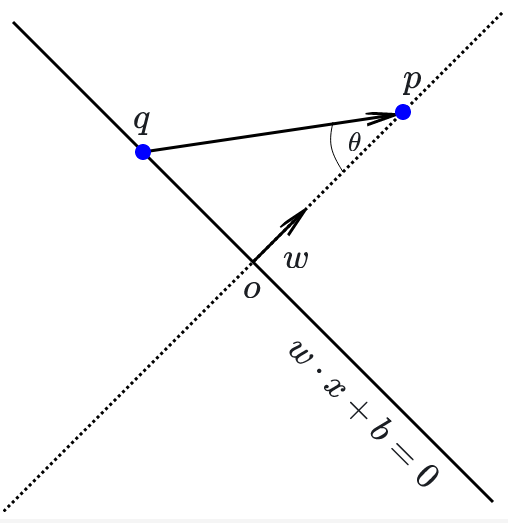
\includegraphics[width=0.3\textwidth,height=\textheight]{../img/triangle.png}
\caption{Distance to a Hyperplane}\label{fig:triangle}
}
\end{figure}

\hypertarget{sec:linearseparable}{%
\subsubsection{Linear separability}\label{sec:linearseparable}}

Now we can return to our classification scheme. The following definition
generalizes our two dimensional picture from the penguin data.

\textbf{Definition:} Suppose that we have an \(n\times k\) data matrix
\(X\) and a set of labels \(Y\) that assign the \(n\) samples to one of
two classes. Then the labelled data is said to be \emph{linearly
separable} if there is a vector \(w\) and a constant \(b\) so that, if
\(f(x)=w\cdot x+b\), then \(f(x)>0\) whenever \(x=(x_1,\ldots, x_k)\) is
a row of \(X\) -- a sample -- belonging to the \(+1\) class, and
\(f(x)<0\) whenever \(x\) belongs to the \(-1\) class. The solutions to
the equation \(f(x)=0\) in this situation form a hyperplane that is
called a \emph{separating hyperplane} for the data.

In the situation where our data falls into two classes that are linearly
separable, our classification strategy is to find a separating
hyperplane \(f\) for our training data. Then, given a point \(x\) whose
class we don't know, we can evaluate \(f(x)\) and assign \(x\) to a
class depending on whether \(f(x)>0\) or \(f(x)<0\).

This definition begs two questions about a particular dataset:

\begin{enumerate}
\def\labelenumi{\arabic{enumi}.}
\tightlist
\item
  How do we tell if the two classes are linearly separable?
\item
  If the two sets are linearly separable, there are infinitely many
  separating hyperplanes. To see this, look back at the penguin example
  and notice that we can `wiggle' the red line a little bit and it will
  still separate the two sets. Which is the `best' separating
  hyperplane?
\end{enumerate}

Let's try to make the first of these two questions concrete. We have two
sets of points \(A\) and \(B\) in \(\mathbf{R}^{k}\), and we want to
(try to) find a vector \(w\) and a constant \(b\) so that
\(f(x)=w\cdot x+b\) takes strictly positive values for \(x\in A\) and
strictly negative ones for \(x\in B\). Let's approach the problem by
first choosing \(w\) and then asking whether there is a \(b\) that will
work. In the two dimensional case, this is equivalent to choosing the
slope of our line, and then asking if we can find an intercept so that
the line passes between the two classes.

In algebraic terms, we are trying to solve the following system of
inequalities: given \(w\), find \(b\) so that: \[
w\cdot x+b>0 \hbox{ for all $x$ in A}
\] and \[
w\cdot x+b<0\hbox{ for all $x$ in B}.
\] This is only going to be possible if there is a gap between the
smallest value of \(w\cdot x\) for \(x\in A\) and the largest value of
\(w\cdot x\) for \(x\in B\). In other words, given \(w\) there is a
\(b\) so that \(f(x)=w\cdot x+b\) separates \(A\) and \(B\) if \[
\max_{x\in B}w\cdot x < \min_{x\in A} w\cdot x.
\] If this holds, then choose \(b\) so that \(-b\) lies in this open
interval and you will obtain a separating hyperplane.

\textbf{Proposition:} The sets \(A\) and \(B\) are linearly separable if
there is a \(w\) so that \[
\max_{x\in B}w\cdot x < \min_{x\in A} w\cdot x
\] If this inequality holds for some \(w\), and \(-b\) within this open
interval, then \(f(x)=w\cdot x+b\) is a separating hyperplane for \(A\)
and \(B\).

\Cref{fig:penguinhwy2} is an illustration of this argument for a subset
of the penguin data. Here, we have fixed \(w=(250,-1)\) coming from the
line \(y=250x+400\) that we eyeballed earlier. For each Gentoo (green)
point \(x_{i}\), we computed \(-b=w\cdot x_{i}\) and drew the line
\(f(x) = w\cdot x - w\cdot x_{i}\) giving a family of parallel lines
through each of the green points. Similarly for each Adelie (blue) point
we drew the corresponding line. The maximum value of \(w\cdot x\) for
the blue points turned out to be \(-75\) and the minimum value of
\(w\cdot x\) for the green points turned out to be \(525\). Thus we have
two lines with a gap between them, and any parallel line in that gap
will separate the two sets.

Finally, among all the lines with this particular \(w\), it seems that
the \textbf{best} separating line is the one running right down the
middle of the gap between the boundary lines. Any other line in the gap
will be closer to either the blue or green set that the midpoint line
is.

\begin{figure}
\hypertarget{fig:penguinhwy2}{%
\centering
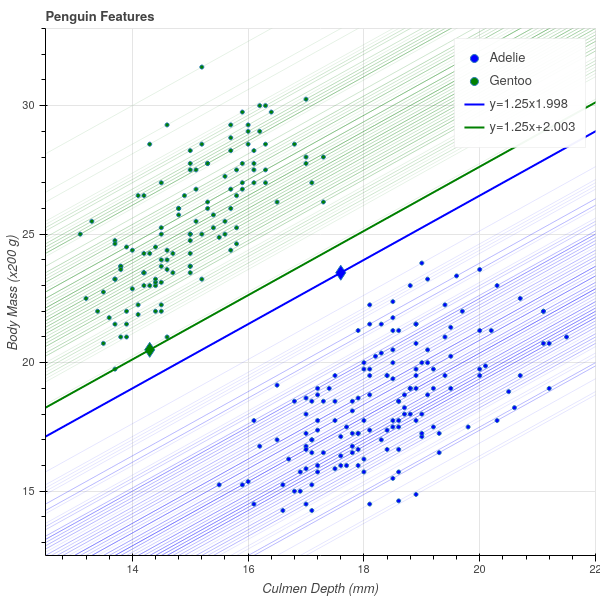
\includegraphics[width=0.5\textwidth,height=\textheight]{../img/penguinhwy2.png}
\caption{Supporting lines in Penguin Data}\label{fig:penguinhwy2}
}
\end{figure}

Let's put all of this together and see if we can make sense of it in
general.

Suppose that \(A^{+}\) and \(A^{-}\) are finite point sets in
\(\mathbf{R}^{k}\) and \(w\in\mathbf{R}^{k}\) such that \[
B^{-}=\max_{x\in A^{-}}w\cdot x < \min_{x\in A^{+}}w\cdot x=B^{+}.
\] Let \(x^{-}\) be a point in \(B\) with \(w\cdot x^{-}=B^{-}\) and
\(x^{+}\) be a point in \(A\) with \(w\cdot x^{+}=B^{+}\). The two
hyperplanes \(f^{\pm}(x) = w\cdot x - B^{\pm}\) have the property that:
\[
f^{+}(x)\ge 0\hbox{ for }x\in A^{+}\hbox{ and }f^{+}(x)<0\hbox{ for }x\in A^{-}
\] and \[
f^{-}(x)\le 0\hbox{ for }x\in A^{-}\hbox{ and }f^{-}(x)>0\hbox{ for }x\in A^{+}
\]

Hyperplanes like \(f^{+}\) and \(f^{-}\), which ``just touch'' a set of
points, are called supporting hyperplanes.

\textbf{Definition:} Let \(A\) be a set of points in \(\mathbf{R}^{k}\).
A hyperplane \(f(x)=w\cdot x+b=0\) is called a \emph{supporting
hyperplane} for \(A\) if \(f(x)\ge 0\) for all \(x\in A\) and \(f(x)=0\)
for at least one point in \(A\), or if \(f(x)\le 0\) for all \(x\in A\)
and \(f(x)=0\) for at least one point in \(A\).

The gap between the two supporting hyperplanes \(f^{+}\) and \(f^{-}\)
is called the \emph{margin} between \(A\) and \(B\) for \(w\).

\textbf{Definition:} Let \(f^{+}\) and \(f^{-}\) be as in the discussion
above for point sets \(A^{+}\) and \(A^{-}\) and vector \(w\). Then the
orthogonal distance between the two hyperplanes \(f^{+}\) and \(f^{-}\)
is called the geometric margin \(\tau_{w}(A^{+},A^{-})\) (along \(w\))
between \(A^{+}\) and \(A^{-}\). We have \[
\tau_{w}(A^{+},A^{-})=\frac{|B^{+}-B^{-}|}{\|w\|}.
\]

\hypertarget{bibliography}{%
\section*{References}\label{bibliography}}
\addcontentsline{toc}{section}{References}

\hypertarget{refs}{}
\begin{cslreferences}
\leavevmode\hypertarget{ref-vapnik92}{}%
{[}1{]} \textsc{Boser}, B., \textsc{Guyon}, I. and \textsc{Vapnik}, V. A
training algorithm for optimal margin classifiers. In \emph{Colt '92:
Proceedings of the fifth annual workshop on computational learning
theory} (D. Haussler, ed) pp 144--52. ACM.

\leavevmode\hypertarget{ref-penguins}{}%
{[}2{]} \textsc{KB}, G., \textsc{TD}, W. and \textsc{WR}, F. (2014).
Ecological sexual dimorphism and environmental variability within a
community of antarctic penguins (genus pygoscelis). \emph{PLoS ONE}
\textbf{9(3)} --13.

\leavevmode\hypertarget{ref-penguindata}{}%
{[}3{]} \textsc{Horst}, A. Palmer penguins.Available at
\url{https://https://github.com/allisonhorst/palmerpenguins}.
\end{cslreferences}

\end{document}
